\section{Feature Representation and Tranferability}
Two common aspects of the sensor points in a building are the actual data readings and the text string-based point names. Both play an important role for differentiating sensor types.
In this section, we elaborate the construction of two different sets of feature vectors (i.e., data features and name features) and empirically discuss how each of them transfers across buidlings in classifying sensor \emph{type}.

\begin{figure*}[ht!]
\centering
  \begin{subfigure}{0.32\textwidth}
                \centering
    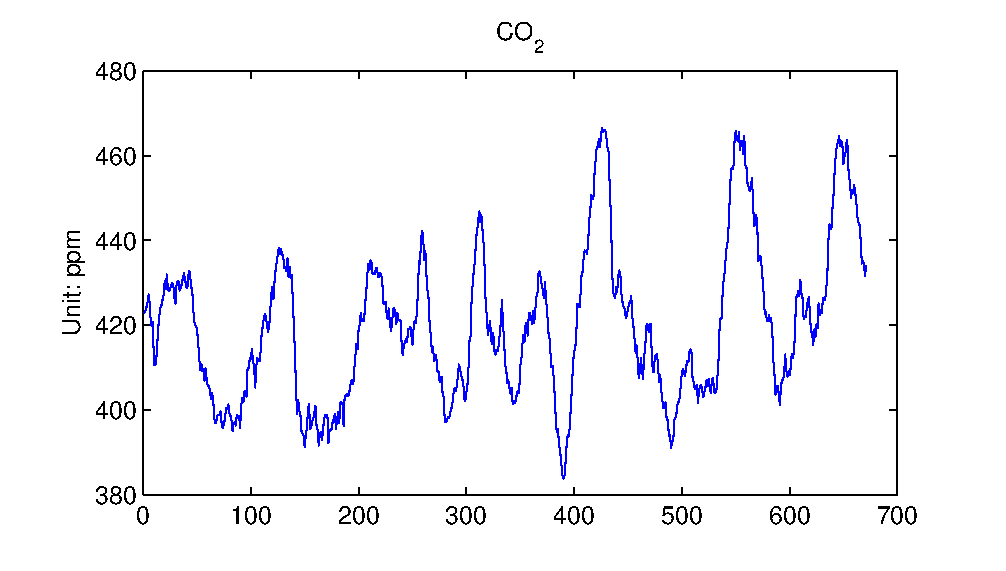
\includegraphics[width=\textwidth]{./fig/co2.eps}
                \caption{$CO_{2}$}
  \end{subfigure}
  \begin{subfigure}{0.32\textwidth}
                \centering
    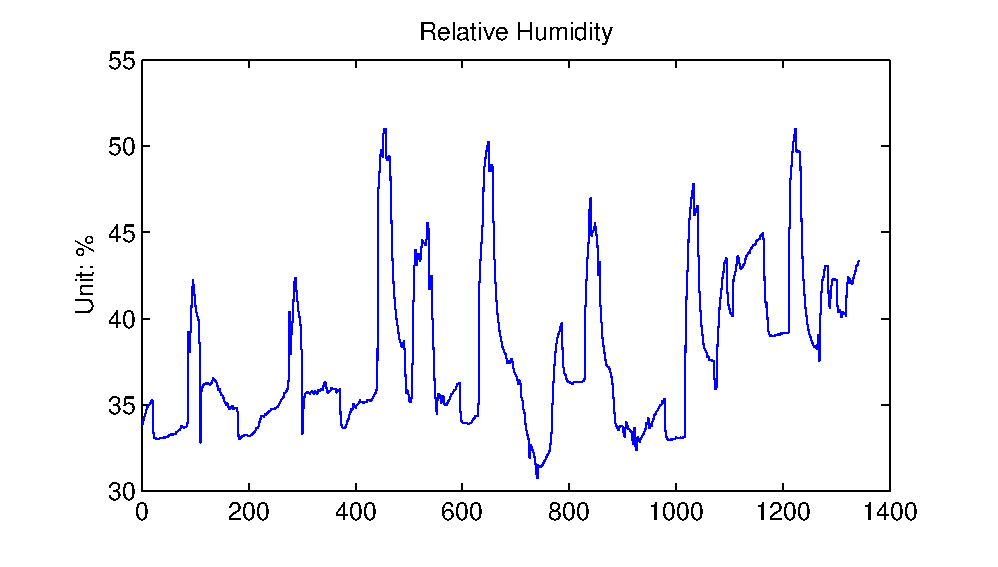
\includegraphics[width=\textwidth]{./fig/rh.eps}
                \caption{Humidity}
  \end{subfigure}
  \begin{subfigure}{0.32\textwidth}
                \centering
    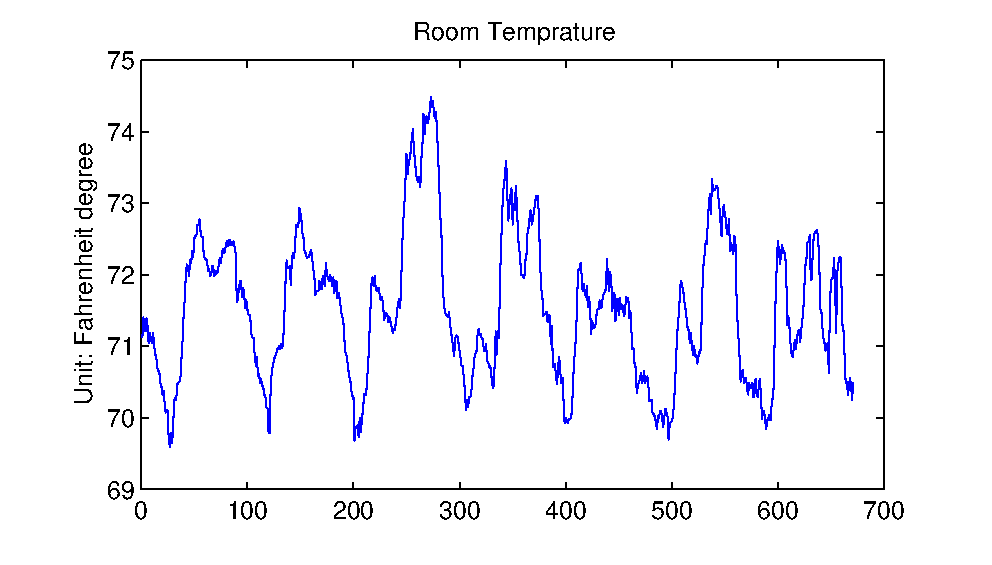
\includegraphics[width=\textwidth]{./fig/rmt.eps}
                \caption{Room Temperature}
  \end{subfigure}
  %row2
  \begin{subfigure}{0.32\textwidth}
                \centering
    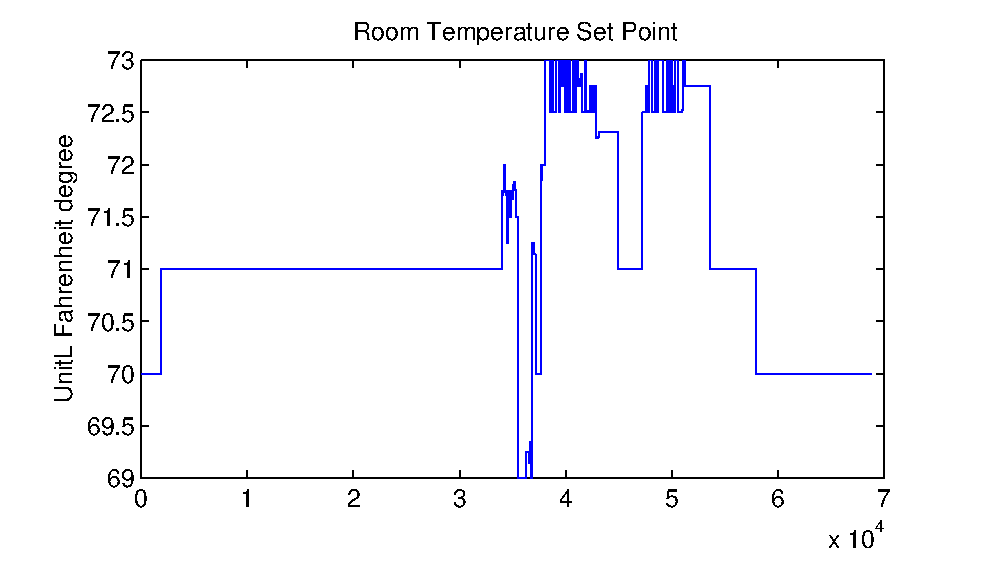
\includegraphics[width=\textwidth]{./fig/stpt.eps}
                \caption{Room Temperature Set Point}
  \end{subfigure}
  \begin{subfigure}{0.32\textwidth}
                \centering
    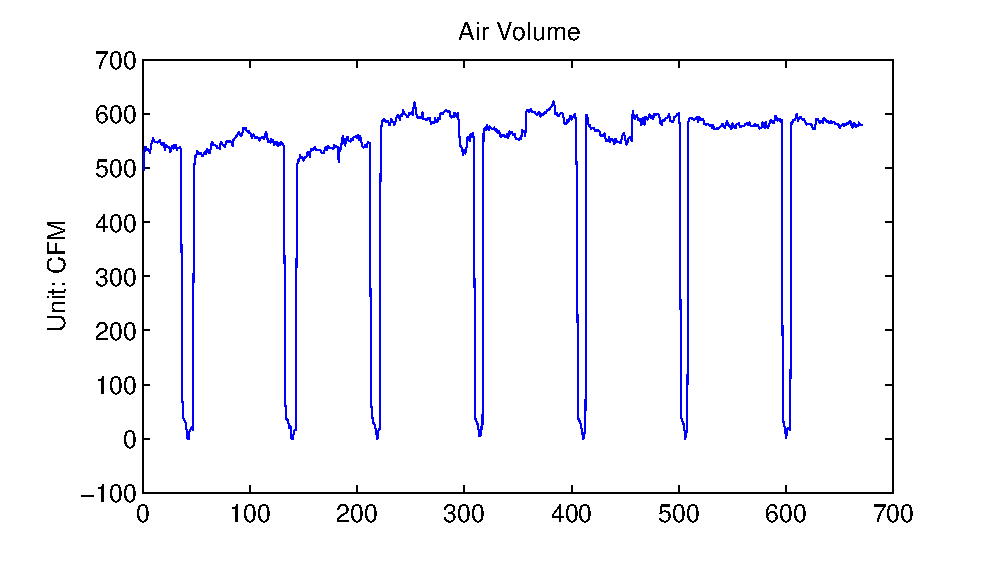
\includegraphics[width=\textwidth]{./fig/vav.eps}
                \caption{VAV Air Volume}
  \end{subfigure}
  \begin{subfigure}{0.32\textwidth}
                \centering
    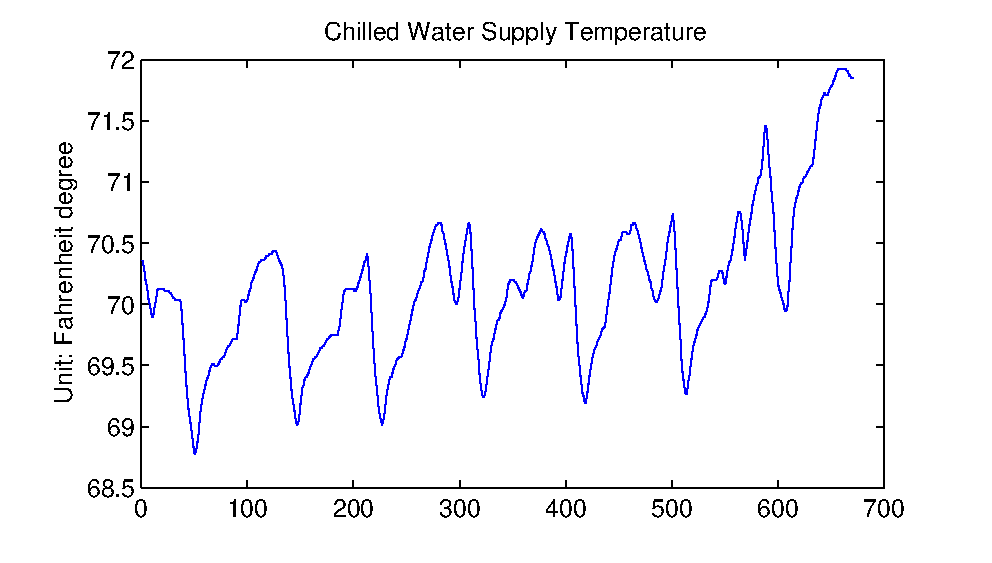
\includegraphics[width=\textwidth]{./fig/cwt.eps}
                \caption{Chilled Water Supply Temperature}
  \end{subfigure}
\caption{Different types of sensors occupy different amplitude bins in the time domain with different short term dynamics.}
\label{fig:example}
\end{figure*}

\subsection{Data Features}
Raw sensor time series\footnote{In this paper, we use the term ``trace'' and ``time series'' \textit{interchangeably}.} usually contain millions of readings which are too many to be useful for type classification. We need to distill the information embedded in the reading patterns.
A signal in the time domain trends the sensor reading and different types of sensor generally occupy distinct amplitude bins, as demonstrated in Figure~\ref{fig:example}. 
We characterize the distribution of a signal in the time domain with standard statistical features, such as the 50th percentile value (also known as the median) as discriminators. 
Table~\ref{table:fd} summarizes the statistical features we used to represent each stream. 


\begin{table}[h]
\centering
\begin{tabular}{r|l|l}
\hline
Category                   & Statistical Funciton & \multicolumn{1}{l}{Acronym} \\ \hline\hline
\multirow{2}{*}{Extreme}   & Minimum                 & min                          \\ \cline{3-3} 
                           & Maximum                 & max                          \\ \hline
\multirow{2}{*}{Average}   & Median                  & emd                          \\ \cline{3-3} 
                           & Root Mean Square        & rms                          \\ \hline
\multirow{2}{*}{Quartiles} & 1st and 3rd Quartiles   & 1q, 3q                       \\ \cline{3-3} 
                           & Inter-quartile range    & iqr                          \\ \hline
\multirow{3}{*}{Moments}   & Variance                & var                          \\ \cline{3-3} 
                           & Skewness                & skew                         \\ \cline{3-3} 
                           & Kurtosis                & kurt                         \\ \hline
Shape                      & Linear Regression Slope & slope                        \\ \hline
\end{tabular}
\caption{Statistical features extracted in window level for each time series data.}
\label{table:fd}
\end{table}


We segment each sensor readings into an hour-long windows and extract the above features within each windsow. 
However, computing features over these short time windows will produce too much information as well as noise; too many feature variables typically degrades classifier performance.
To succinctly summarize the dynamics of sensor traces, we compute the statistics of the accumulated features from windowed slices as the final feature set. 
We construct our feature vector as follows: first, each sensor trace is segmented into N non-overlapping one-hour long windows. Second, within each time window, we compute the statistics as in the above table for the trace, producing a vector of each statistical feature after the window slides over the entire trace, such as 
$MIN = \{min^{1}, min^{2}, ..., min^{N}\}$, where N is the number of time windows. Each vector (such as this $MIN$) reflects short term changes but not all the intermediate values are useful for classification. 
Finally, we compute a statistical summary of these vectors. For each vector we compute the minimum, maximum, median and variance, resulting in a feature vector containing 44 variables:
\begin{displaymath}
\begin{split}
F = \{min(MIN), max(MIN), median(MIN), var(MIN),\\
...\\
min(SLOPE), max(SLOPE), median(SLOPE), var(SLOPE)\}
\end{split}
\end{displaymath}
$F$ is the data feature vector for each sensor trace used in our study.


\subsection{Name Features}
The sensor point names are short text strings with several concatenated abbreviations, as shown in our motivating example in Table~\ref{table:ex}. 
To represent the primitive point names as feature vectors for classifier training, we first convert all point names to lower cases and trim out the numerical characters in each point name, resulting in a series of words, e.g., \texttt{Zone Temp 2 RMI204} becomes \texttt{\{zone, temp, rmi\}}. 
To capture possible variants of abbreviations in point names, e.g., ``tmp'' and ``temp'' for temperature, we adopt $k$-mers \cite{leslie2004mismatch} as our features. 
The term $k$-mer refers to all the possible substrings of length $k$, which are contained in a string. This feature is popularly used in protein and gene sequence analysis in bioinformatics, and it helps measure sequence similarity without requiring alignment. 

In our case, we limit the k-mers computation only within a word boundary.
In general, having a too small $k$ will increase the chance for all the k-mers to overlap, making all the points less differentiable.
Therefore, we compute all k-mers of length 3 and 4 for each point name.
For example, \texttt{\{zone, temp, rmi\}} will yield a set of k-mers \texttt{\{zon, one, tem, emp, rmi\}} with $k$=3.
A dictionary of k-mers is constructed with all the k-mers generated from each point name. 
Each point name is converted into a feature vector based on the frequency of k-mers in it. 
For example, a set of k-mers \texttt{\{zon, tem, emp, zon\}} will be transformed to a vector
\texttt{(2,0,1,1,0)} with the dictionary \texttt{\{zon, one, tem, emp, rmi\}}, meaning \texttt{zon} occurs twice, \texttt{one} doesn't appear, and so forth. 
This feature representation of point names will be used for examining classification performance.

\subsection{Transferability}
Now with the two differet types of features explained, we examine how well both can perform in classifying sensor types when applied across buildings, i.e., learning a classifier based on the features from building A and testing it on building B. 
Intuitively, data features should be more generalizable than point names with respect to differentiating points by types. 
This is because in general a certain type of sensors will share commonatiliteis in reading amplitude and trend, such as diurnal patterns. 
For exmaple, temperature readings in a building will be between 60-70 degree with rises in the morning and falls at night.
In contrast, point name features might not transfer well due to various naming conventions across buildings as shown in Table~\ref{table:ex}.
Although k-mers can enlarge the size of term dictionary in a building to increase the chance of covering more terms in other buildings, such a technique still cannot fundamentally compensate for the difference in naming conventions.

\begin{table}[h]
\centering
\begin{tabular}{l|c|c}
\hline
                & Data Feature & Name Feature \\ \hline
A-\textgreater B & 77.8\%       & 34.1\%       \\
B-\textgreater A & 61.2\%       & 32.8\%       \\ \hline
\end{tabular}
\caption{Type Classification Accuracy between Building A\&B with Different Features.}
\label{table:clf}
\end{table}


To empirically examine how well each type of feature transfers, we perform type classification across buildings with both features in separate. With either set of features from building A, we train a linear SVM and apply it to building B on the same type of feature, or vice versa. Table~\ref{table:clf} summarizes the results.
We see that data features do transfer better than name features as expected, but the results from data features still contain significant errors making them far from being usable. 
The question remains how to better leverage these two sources of information from one building and transfer them to another.
We will discuss the idea of transfer learning in next section.

